\documentclass[a4paper,11pt]{article}
\usepackage{graphicx} % Required for inserting images
\usepackage[portuguese]{babel}

\title{BD-PL05}
\author{Eduardo Freitas Fernandes}
\date{2025}

\begin{document}

\maketitle

\noindent \textbf{Exercício 1}\\

\noindent A Federação de Desporto de Bragança é uma organização que cria eventos desportivos para vários atletas participarem. Esta organização trabalha em conjunto com os vários Clubes a que os desportistas pertencem. De forma a escalar os eventos, a federação decidiu implementar um sistema de base de dados para conseguir organizar as provas feitas e a informação relativa aos atletas que nelas participam.\\

\noindent \textbf{Exercício 2}\\

\noindent Lista de requisitos de Descrição:

\begin{itemize}
    \item Cada \textbf{clube} terá um registo único, através de um identificador. É acompanhado pelo nome do seu presidente, a sua designação e o número de atletas que tem.
    \item Todos os \textbf{atletas} têm um número único, a sua data de nascimento, o local onde nasceram e o nome do seu treinador.
    \item Uma \textbf{modalidade} é representada através de um identificador único e uma breve descrição.
    \item Todas as \textbf{provas} devem ser identificadas pelo um id único. Devem conter informação sobre o local onde foi realizada, a data e os patrocinadores. Deve também ter uma designação e uma referência ao diretor da prova.
    \item As \textbf{participações} numa prova devem ter um prémio associado à classificação do atleta.
\end{itemize}

\noindent \textbf{Exercício 3}\\

\noindent Analisando o esquema conceptual apresentado, podemos construir o esquema lógico seguinte:

\newpage

\begin{figure}[h]
    \centering
    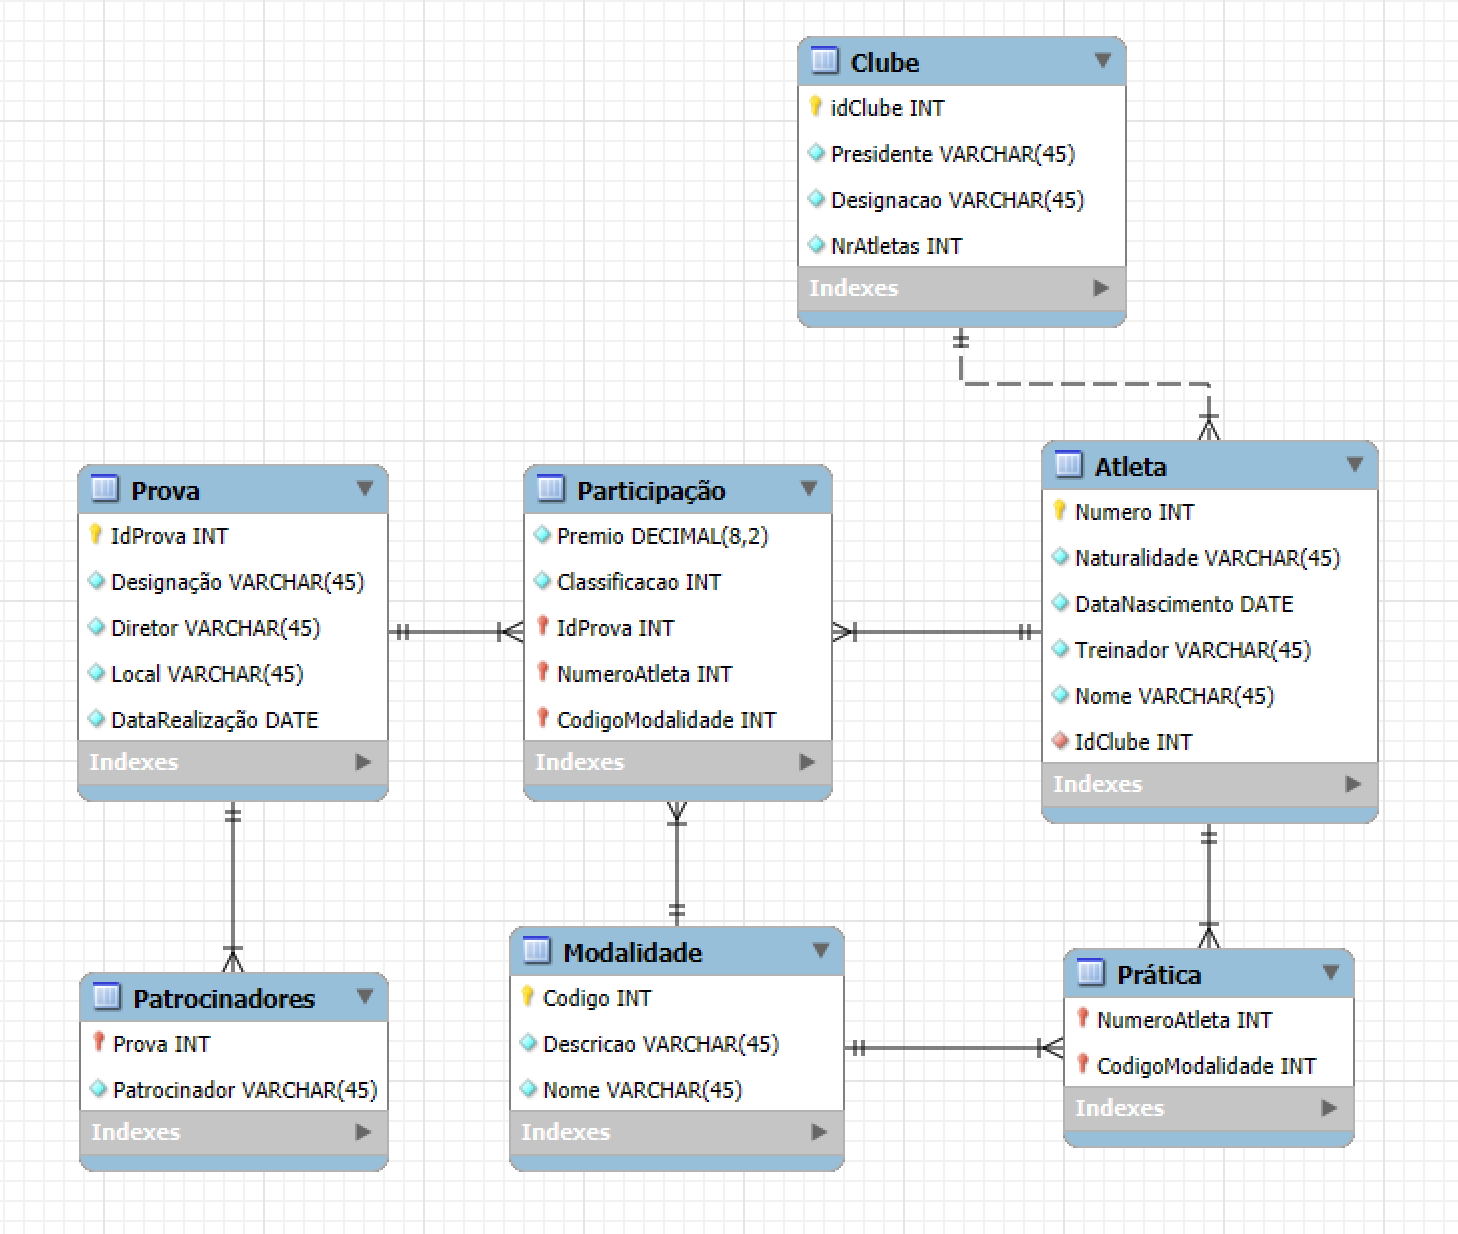
\includegraphics[width=1\linewidth]{imgs/pl05-esquema_logico.png}
    \caption{Esquema Lógico}
\end{figure}

\noindent \textbf{Exercício 4}\\

\noindent O campo \texttt{NrAtletas} na tabela \texttt{Clubes} é algo que pode ser calculado através de uma query, logo poderá ser um valor repetitivo. O campo \texttt{Treinador} na tabela \texttt{Atletas} não parece ser dependente de um atleta, logo poderia ser uma entidade nova. Mesma situação se aplica para o \texttt{Presidente} de um clube.

\newpage
\noindent \textbf{Exercício 5}\\

\begin{figure}[h]
    \centering
    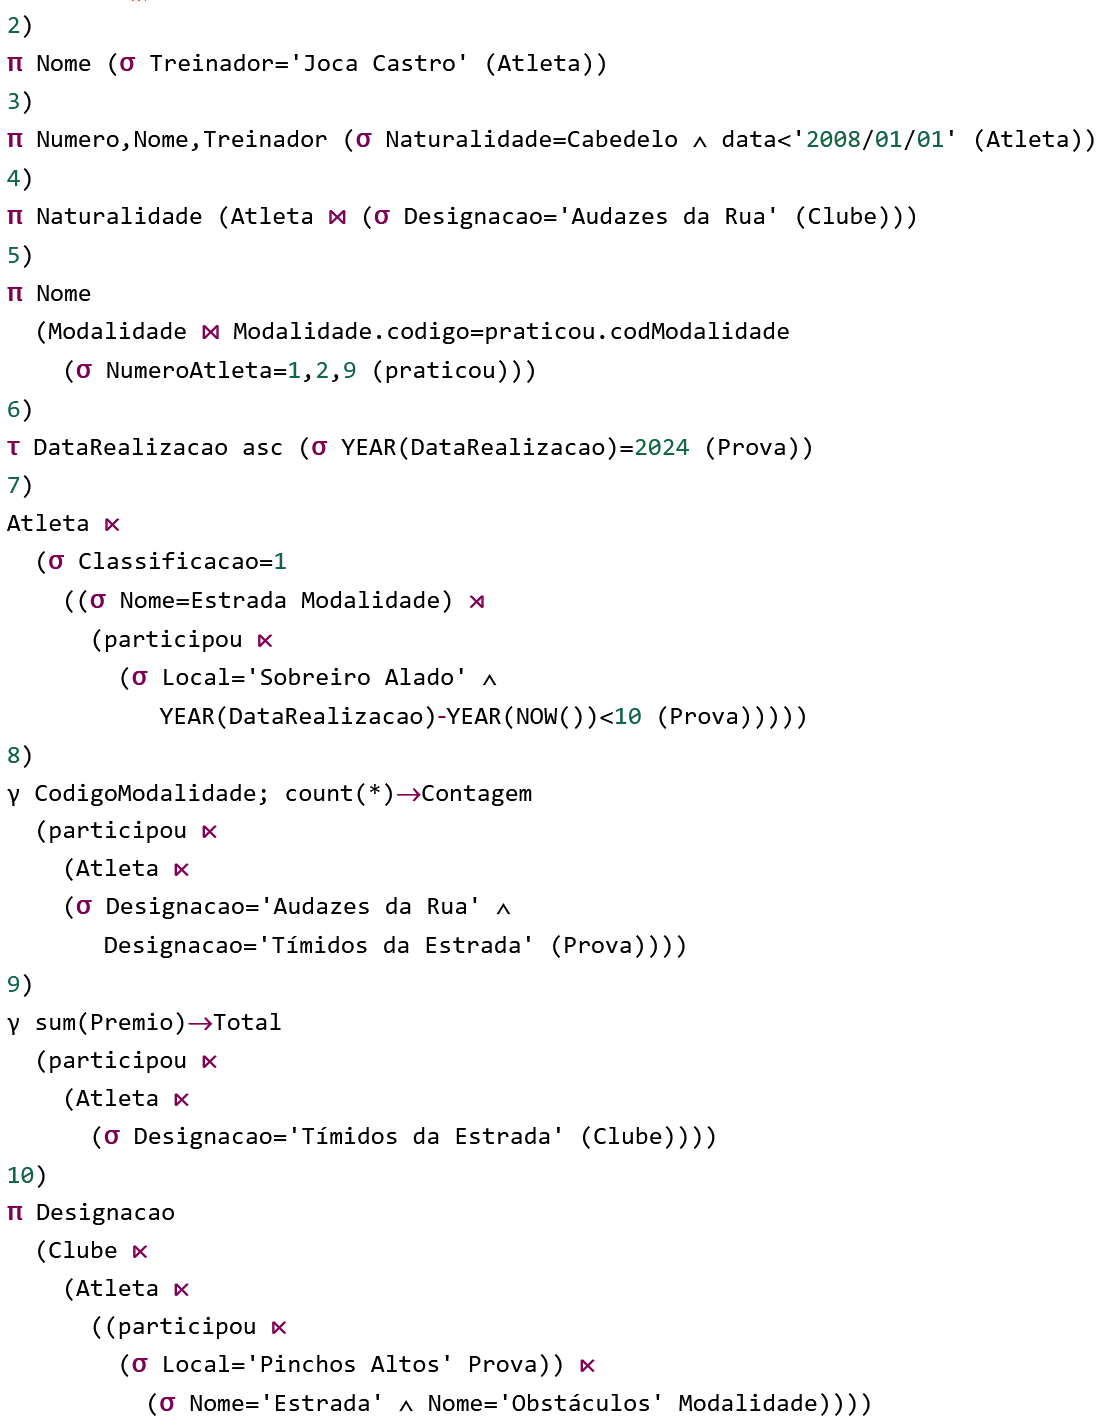
\includegraphics[width=0.95\linewidth]{imgs/exercicio-e.png}
    \caption{Expressões de Algebra Relacional}
\end{figure}



\end{document}
